\documentclass[graduacao,brazilian]{thesispuc}



%%%
%%% Additional Packages
%%%
\usepackage{tabularx}
\usepackage{multirow}
\usepackage{multicol}
\usepackage{colortbl}
\usepackage[%
    dvipsnames,
    svgnames,
    x11names,
    fixpdftex,
    table
]{xcolor}
\usepackage{numprint}
\usepackage{textcomp}
\usepackage{booktabs}
\usepackage{amsmath}
\usepackage{enumitem}
\usepackage{amssymb}

\usepackage[alf,bibjustif,abnt-emphasize=bf]{abntex2cite}
%\usepackage{tikz}
%\usepackage[linesnumbered, ruled, vlined]{algorithm2e}
%\usepackage{pgfplots,pgfplotstable}
%\usepackage{array} 

%% numprint
\npthousandsep{.}
\npdecimalsign{,}

%% ThesisPUC option
\tablesmode{tab}        %% listas de figuras e de tabelas [nada, fig, tab ou figtab]
\algorithmsmode{none}      %% lista de algoritmos [none ou use]
\codesmode{none}           %% lista de códigos [none ou use]
\abreviationsmode{none}    %% lista de abreviaturas [none ou use]


%%%
%%% Counters
%%%

%% uncomment and change for other depth values
\setcounter{tocdepth}{1}
%\setcounter{lofdepth}{3}
%\setcounter{lotdepth}{3}
%\setcounter{secnumdepth}{3}

%%%
%%% Misc.
%%%

\usecolour{true}


%%%
%%% Identificação (capa, folha de rosto, resumo)
%%%

\author{Gabriel Lobo de Sant'Anna Rosas}
\authorR{Lobo de Sant'Anna Rosas, Gabriel} % Sobrenomes, Nome

\advisor{Adriano Francisco Branco}{}       % Nome Sobrenome
\advisorR{Francisco Branco, Adriano}       % Sobrenome, Nome

\coadvisor{Jonatas dos Santos Grosman}{}
\coadvisorR{dos Santos Grosman, Jonatas}

\title{Alocação preditiva de recursos em nuvem via previsão de carga com Redes Neurais para minimização de custos operacionais}
\titleuk{Predictive cloud resource allocation via workload forecasting with neural networks for operating cost minimization}
%\subtitle{Subtítulo, se houver}

\day{\day}
\month{Novembro}
\year{2026}

\city{Rio de Janeiro}
\university{Pontifícia Universidade Católica do Rio de Janeiro}
\school{Centro Técnico Científico - CTC}
\department{Informática}
\program{Engenharia da Computação} 
% \curso{Engenharia da Computação}              % Curso de Graduação em ...
% \titulacao{Engenheiro de Computação}          % título a ser obtido
% \disciplina{Projeto Final I}{Undergraduate Thesis I}


 
\keywords{%
  \key{Computação em nuvem}
  \key{Alocação de recursos}
  \key{Previsão de carga}
  \key{Redes neurais}
  \key{Acordo de nível de serviço}
}

\keywordsuk{%
  \key{Cloud computing}
  \key{Resource allocation}
  \key{Workload forecasting}
  \key{Neural networks}
  \key{Service level agreement}
}


\abstract{%
Provedores de nuvem precisam decidir continuamente quantas instâncias manter ativas: recursos em excesso elevam o custo, e recursos insuficientes violam o acordo de nível de serviço. A alocação reativa só ajusta a capacidade depois de observar a mudança na demanda e, por isso, chega atrasada nos picos. Este trabalho investiga o quanto a qualidade da previsão de carga reduz o custo de alocação sem aumentar as violações de serviço. Para atribuir as diferenças ao previsor, a política de alocação é mantida fixa e apenas o previsor muda. São comparados métodos tradicionais de previsão (ingênuo, média móvel, sazonal, Holt-Winters e ARIMA) e uma rede neural recorrente do tipo GRU, além de uma política reativa e de um dimensionamento estático no pico, sobre séries de utilização agregadas a partir do rastro público de um aglomerado da Alibaba e avaliadas em um centro de dados simulado. As métricas são o custo normalizado pelo de um oráculo e a fração de intervalos com violação. Os resultados preliminares mostram que a previsão reduz muito o custo frente ao dimensionamento estático e de forma modesta frente à política reativa, e que a GRU é competitiva com o ARIMA, sem vantagem clara. Esta etapa também define o ambiente e o plano do Projeto Final II.%
}

\abstractuk{%
Cloud providers must continuously decide how many instances to keep active: excess resources raise costs, while insufficient resources violate the service level agreement. Reactive allocation adjusts capacity only after observing a change in demand and therefore lags behind peaks. This work investigates how much the quality of workload forecasting reduces allocation cost without increasing service violations. To attribute differences to the forecaster, the allocation policy is kept fixed and only the forecaster changes. Traditional forecasting methods (naive, moving average, seasonal, Holt-Winters and ARIMA) and a recurrent neural network of the GRU type are compared, together with a reactive policy and a static peak sizing, using utilization series aggregated from a public Alibaba cluster trace and evaluated in a simulated data center. The metrics are the cost normalized by that of an oracle and the fraction of intervals with violations. Preliminary results show that forecasting greatly reduces cost compared with static sizing and only modestly compared with the reactive policy, and that the GRU is competitive with ARIMA, with no clear advantage. This stage also defines the environment and the plan for the second part of the project.%
}

\begin{document}
  \chapter{Introdução}
\label{cap:introducao}

\section{Motivação}
\label{sec:motivacao}

A computação em nuvem consolidou-se como a principal forma de disponibilizar infraestrutura computacional para empresas e instituições. Nesse modelo, o provedor mantém grandes centros de dados e precisa decidir, de forma contínua, quanto de processamento, memória e armazenamento deve estar disponível para atender à demanda de seus clientes. Como a demanda tende a crescer, impulsionada sobretudo por aplicações de Inteligência Artificial e de análise de grandes volumes de dados, a gestão eficiente desses recursos tornou-se um fator central para a sustentabilidade econômica dos provedores \cite{rossi2023forecasting}.

A dificuldade está no fato de que a carga de trabalho não é constante. Ela apresenta picos, padrões periódicos e variações aparentemente aleatórias. Diante disso, a abordagem mais comum é a alocação reativa, na qual o sistema ajusta os recursos apenas depois de observar uma mudança na demanda, normalmente por meio de regras de limiar sobre a utilização. Como a reação ocorre com atraso, esse tipo de estratégia tende a degradar o desempenho durante os picos e a desperdiçar recursos nos períodos de baixa utilização \cite{bodra2025ml}.

Esse cenário cria um dilema permanente. Manter recursos em excesso (superprovisionamento) garante a qualidade do serviço, mas eleva o custo operacional. Manter recursos de menos (subprovisionamento) reduz o custo, mas provoca violações dos Acordos de Nível de Serviço (\textit{Service Level Agreements}, SLA) firmados com os clientes. Uma alternativa é a alocação preditiva, que utiliza o histórico de uso para antecipar a demanda futura e provisionar recursos antes que eles sejam necessários \cite{bodra2025ml}. Nesse contexto, prever a carga com precisão passa a ser uma pré-condição para otimizar a alocação \cite{rossi2023forecasting}.

A previsão de carga em nuvem foi tradicionalmente tratada com modelos estatísticos lineares, como o modelo autorregressivo integrado de médias móveis (ARIMA) \cite{calheiros2015arima}. Mais recentemente, redes neurais profundas, em especial as arquiteturas recorrentes, passaram a ser aplicadas ao problema com bons resultados, inclusive em abordagens multivariadas que consideram simultaneamente o uso de processador e de memória \cite{xu2022esdnn}.

\section{Definição do problema}
\label{sec:definicao-problema}

O problema tratado neste trabalho tem duas partes encadeadas. A primeira é um problema de previsão: dado o histórico de utilização de recursos de um \textit{cluster}, amostrado em intervalos regulares, estimar a demanda de processador e de memória em um horizonte curto. A segunda é um problema de decisão: a partir dessa estimativa, determinar quantas instâncias de recursos (máquinas virtuais ou contêineres) devem permanecer ativas em cada intervalo.

De forma preliminar, a decisão pode ser formulada como a minimização do custo operacional sujeita a uma restrição de qualidade de serviço:

\begin{equation}
\label{eq:problema}
\min_{n_1, \dots, n_T} \; \sum_{t=1}^{T} c \cdot n_t
\quad \text{sujeito a} \quad
\frac{1}{T} \sum_{t=1}^{T} \mathbf{1}\left[\, d_t > k \cdot n_t \,\right] \leq \varepsilon,
\end{equation}

\noindent em que $n_t$ é o número de instâncias ativas no intervalo $t$, $c$ é o custo de uma instância por intervalo, $k$ é a capacidade de uma instância, $d_t$ é a demanda real observada, $\mathbf{1}[\cdot]$ é a função indicadora e $\varepsilon$ é a fração máxima de intervalos com violação de SLA tolerada. Como $d_t$ não é conhecida no momento da decisão, a escolha de $n_t$ depende da previsão $\hat{d}_t$, e a qualidade dessa previsão afeta diretamente o custo e o número de violações. Essa formulação é refinada no Capítulo~\ref{cap:objetivos}, que define como a restrição é verificada na prática (Equação~\ref{eq:calibracao}).

\section{Justificativa}
\label{sec:justificativa}

A relevância do problema é econômica e operacional. Cada ponto percentual de recursos ociosos representa custo para o provedor, e cada violação de SLA representa perda de qualidade percebida pelo cliente e, eventualmente, penalidades contratuais. Apesar do volume de trabalhos sobre previsão de carga, falta uma avaliação de ponta a ponta, com dados públicos, que meça quanto a previsão reduz o custo de alocação quando redes neurais e métodos tradicionais são submetidos à mesma política, lacuna discutida na Seção~\ref{sec:lacuna}.

\section{Escopo e delimitação}
\label{sec:escopo}

\textbf{Incluído.} Rastros públicos da Alibaba \cite{alibaba2018trace} e do Google \cite{wilkes2020google}, agregados em séries de uso de processador e de memória; horizontes de previsão curtos, na escala de minutos; alocação em um centro de dados simulado, com custo por instância ativa e violação de SLA nos intervalos em que a demanda excede a capacidade; e comparação entre uma rede neural e métodos tradicionais de previsão sob a mesma política de alocação, ao lado das políticas de referência da Seção~\ref{sec:solucao}.

\textbf{Fora do escopo.} Implantação em uma nuvem real, posicionamento e migração de máquinas virtuais entre servidores físicos, consumo de energia, múltiplos provedores e aprendizado por reforço para a decisão. Na simulação, o posicionamento segue a política padrão do simulador, a mesma para todos os previsores.

\section{Organização do documento}
\label{sec:organizacao}

O restante deste documento está organizado da seguinte forma. O Capítulo~\ref{cap:situacao-atual} apresenta a terminologia básica e as principais abordagens existentes para previsão de carga e alocação de recursos em nuvem, com suas limitações, além das tecnologias utilizadas. O Capítulo~\ref{cap:objetivos} descreve a solução proposta, seus objetivos específicos e o que será efetivamente implementado. O Capítulo~\ref{cap:plano-acao} revisa o plano de ação, comparando as atividades previstas com as realizadas, e apresenta os resultados preliminares do protótipo. Por fim, o Capítulo~\ref{cap:cronogramas} apresenta os cronogramas do Projeto Final I (PF~I) e do Projeto Final II (PF~II).
  \chapter{Situação Atual}
\label{cap:situacao-atual}

Este capítulo apresenta o contexto necessário para compreender o problema tratado neste trabalho. A Seção~\ref{sec:conceitos} define os conceitos e a terminologia básica. As Seções~\ref{sec:previsao} e~\ref{sec:alocacao} descrevem, respectivamente, as abordagens existentes para previsão de carga e para alocação de recursos em nuvem, destacando suas limitações. A Seção~\ref{sec:lacuna} compara os trabalhos mais próximos desta proposta, e a Seção~\ref{sec:tecnologias} apresenta as tecnologias utilizadas.

\section{Conceitos e terminologia}
\label{sec:conceitos}

\subsection{Elasticidade, carga de trabalho e séries temporais}
\label{subsec:carga}

Uma das características essenciais da computação em nuvem é a elasticidade rápida, isto é, a capacidade de provisionar e liberar recursos rapidamente, em alguns casos de forma automática, acompanhando a demanda \cite{mell2011nist}. \citeonline{herbst2013elasticity} definem elasticidade como o grau em que um sistema se adapta a mudanças na carga de trabalho, provisionando e liberando recursos de forma autônoma, de modo que, a cada instante, os recursos disponíveis correspondam o mais fielmente possível à demanda corrente. Essa definição deixa claro que a elasticidade tem duas falhas possíveis: oferecer recursos de mais ou recursos de menos.

A carga de trabalho (\textit{workload}) de um \textit{cluster} é o conjunto de demandas submetidas a ele, como tarefas em lote, serviços de longa duração e requisições de usuários. Do ponto de vista da infraestrutura, essa carga se manifesta como utilização de recursos, principalmente processador e memória. Quando essa utilização é agregada em intervalos regulares de duração $\Delta$, obtém-se uma série temporal $y_1, y_2, \dots, y_t$, em que $y_t$ é a utilização média (ou máxima) no intervalo $t$. Séries de carga em nuvem costumam combinar tendência, padrões periódicos (por exemplo, diários e semanais), ruído e picos abruptos, o que torna sua previsão difícil \cite{xu2022esdnn}.

Prever a carga significa estimar $\hat{y}_{t+h}$, o valor da série $h$ intervalos à frente, a partir de uma janela com as $w$ observações mais recentes. O parâmetro $h$ é o horizonte de previsão e $w$ é o tamanho da janela de entrada. Quando é preciso distinguir o intervalo em que a previsão é feita do intervalo previsto, o primeiro é chamado de origem da previsão e denotado por $\tau$: uma previsão feita na origem $\tau$ só pode usar observações até $\tau$. A previsão é univariada quando usa apenas a própria série e multivariada quando incorpora outras séries correlacionadas, como prever o uso de processador a partir do histórico de processador e de memória \cite{xu2022esdnn}.

Pesquisas sobre o tema dependem de rastros (\textit{traces}) públicos de \textit{clusters} reais, que registram eventos e uso de recursos de máquinas, tarefas e contêineres. O rastro mais recente do Google cobre oito células do gerenciador Borg durante o mês de maio de 2019 \cite{wilkes2020google}. O rastro de 2018 da Alibaba cobre cerca de 4.000 máquinas de um \textit{cluster} de produção ao longo de oito dias, com serviços \textit{online} e tarefas em lote compartilhando as mesmas máquinas, e inclui tabelas de uso de recursos por máquina e por contêiner \cite{alibaba2018trace}. Como esses rastros registram eventos e medições em granularidade fina, transformá-los em séries temporais regulares é uma etapa de pré-processamento necessária, que faz parte deste trabalho.

A granularidade dessa agregação varia entre os trabalhos, mas intervalos de cinco minutos são os mais usados com esses rastros. \citeonline{rossi2023forecasting} agregam os rastros do Google e da Alibaba em intervalos de cinco minutos e preveem a demanda dez minutos à frente, horizonte que consideram suficiente para a maioria das aplicações de alocação. O esDNN também adota cinco minutos como intervalo de previsão e de decisão na simulação de escalonamento \cite{xu2022esdnn}. Trabalhos com outros tipos de dado usam escalas diferentes, como uma hora para requisições a servidores \textit{web} \cite{calheiros2015arima} ou um minuto para dados de produção de um provedor \cite{pan2023magicscaler}. O ponto comum é que o intervalo deve ser longo o bastante para que uma nova instância possa ser iniciada dentro dele \cite{calheiros2015arima}.

\subsection{Acordos de nível de serviço}
\label{subsec:sla}

A qualidade de um serviço em nuvem é expressa por três conceitos relacionados \cite{beyer2016sre}. Um indicador de nível de serviço (\textit{Service Level Indicator}, SLI) é uma medida quantitativa de algum aspecto do serviço, como latência, disponibilidade ou fração de requisições atendidas com sucesso. Um objetivo de nível de serviço (\textit{Service Level Objective}, SLO) é um valor-alvo ou uma faixa aceitável para um SLI, por exemplo, atender 99\% das requisições dentro de um limite de tempo. Por fim, um acordo de nível de serviço (\textit{Service Level Agreement}, SLA) é o contrato entre provedor e cliente que formaliza esses objetivos e define as consequências, geralmente financeiras, de não cumpri-los.

Na literatura de alocação de recursos, a violação de SLA é frequentemente aproximada por medidas derivadas da utilização, já que os rastros públicos não registram a latência percebida pelos usuários. \citeonline{beloglazov2012optimal}, por exemplo, medem a fração do tempo em que os servidores ativos operam com utilização máxima, situação em que o desempenho das aplicações é presumivelmente degradado. \citeonline{rossi2023forecasting} consideram atendida a demanda que fica abaixo da capacidade prevista.

Este trabalho adota uma aproximação do mesmo tipo. O SLI é medido por intervalo: o intervalo $t$ é atendido integralmente quando a capacidade disponível cobre a demanda real, isto é, quando $d_t \leq k \cdot n_t$, na notação da Equação~\ref{eq:problema}, e há violação no caso contrário. O SLO correspondente é que no máximo uma fração $\varepsilon$ dos intervalos fique sem atendimento integral, que é exatamente a restrição daquela equação. A fração da demanda que deixa de ser atendida é acompanhada como métrica complementar (Seção~\ref{subsec:metricas}). Essa simplificação não captura efeitos como filas ou degradação gradual de desempenho perto da saturação, mas permite comparar estratégias de alocação de forma consistente e reproduzível.

\subsection{Provisionamento reativo e preditivo}
\label{subsec:provisionamento}

O escalonamento automático (\textit{autoscaling}) é o mecanismo que ajusta os recursos alocados a uma aplicação sem intervenção humana. Ele pode ser horizontal, quando altera o número de instâncias (máquinas virtuais ou contêineres), ou vertical, quando altera a capacidade de cada instância. Este trabalho trata apenas do escalonamento horizontal.

\citeonline{lorido2014autoscaling} classificam as técnicas de escalonamento automático em cinco famílias: regras baseadas em limiares, aprendizado por reforço, teoria de filas, teoria de controle e análise de séries temporais. Do ponto de vista deste trabalho, a distinção mais importante é entre abordagens reativas e preditivas. No provisionamento reativo, a decisão no instante $t$ é tomada a partir do que já foi observado, normalmente a utilização corrente. No provisionamento preditivo, a decisão é tomada a partir de uma estimativa $\hat{d}_{t+h}$ da demanda futura. Na alocação, a série prevista é a própria demanda, isto é, $y_t = d_t$.

A desvantagem da abordagem reativa é o atraso. Entre a detecção de um aumento de carga e a disponibilidade de uma nova instância há o atraso de inicialização, que não é desprezível e varia entre provedores e configurações \cite{mao2012startup}. Durante esse período, a aplicação opera com capacidade insuficiente. Por isso, a decisão de alocação precisa ser tomada com antecedência. Neste trabalho, a decisão tomada com as observações disponíveis até o intervalo $\tau$ passa a valer no intervalo $\tau + L$, em que $L$ é a antecedência da decisão (\textit{lead time}), igual a um intervalo mais o atraso de inicialização, também medido em intervalos. Sem atraso de inicialização, $L = 1$ e a decisão vale já no intervalo seguinte. As duas abordagens estão sujeitas à mesma antecedência: a reativa decide em $\tau$ com a utilização observada em $\tau$, e a preditiva tenta antecipar a demanda do intervalo $\tau + L$, de modo que a instância já esteja disponível quando a carga chegar. Provedores comerciais já oferecem modos de escalonamento preditivo, como o do Amazon EC2 Auto Scaling \cite{aws2024predictive}, o que reforça a relevância prática do problema.

Qualquer que seja a abordagem, cada decisão pode errar em duas direções. Há superprovisionamento quando a capacidade alocada excede a demanda ($k \cdot n_t > d_t$): o serviço é atendido, mas a capacidade ociosa $k \cdot n_t - d_t$ representa custo sem retorno. Há subprovisionamento quando a capacidade é menor que a demanda ($k \cdot n_t < d_t$): o custo é menor, mas parte da demanda não é atendida e o SLA pode ser violado. O objetivo da alocação é equilibrar essas duas falhas, e a qualidade da previsão determina o quanto esse equilíbrio pode ser alcançado.

\subsection{Métricas de avaliação}
\label{subsec:metricas}

As métricas usadas na literatura se dividem em dois grupos, e a distinção entre eles é central para este trabalho.

\textbf{Métricas de previsão.} Medem o quanto a previsão se aproxima do valor real, independentemente de como ela será usada. Para $N$ previsões $\hat{y}_i$ e valores reais $y_i$, as mais comuns são o erro quadrático médio (MSE), sua raiz (RMSE), o erro absoluto médio (MAE) e o erro percentual absoluto médio (MAPE):

\begin{align}
\mathrm{MSE}  &= \frac{1}{N}\sum_{i=1}^{N}(y_i - \hat{y}_i)^2, &
\mathrm{RMSE} &= \sqrt{\mathrm{MSE}}, \label{eq:mse-rmse}\\
\mathrm{MAE}  &= \frac{1}{N}\sum_{i=1}^{N}\lvert y_i - \hat{y}_i \rvert, &
\mathrm{MAPE} &= \frac{100\%}{N}\sum_{i=1}^{N}\left\lvert \frac{y_i - \hat{y}_i}{y_i} \right\rvert. \label{eq:mae-mape}
\end{align}

O MAPE é indefinido quando algum $y_i$ é zero e instável quando $y_i$ é próximo de zero, situação comum em períodos de baixa utilização. Neste trabalho, ele é calculado apenas sobre os pontos em que $y_i$ não é próximo de zero, e a fração de pontos mantida, chamada de cobertura da máscara, é informada junto com o valor. Além disso, as quatro métricas são simétricas: superestimar e subestimar a demanda pela mesma quantidade produz o mesmo erro. Para a alocação, porém, esses erros têm consequências diferentes, já que a superestimação gera custo e a subestimação gera violações. Por isso, um modelo com menor RMSE não é necessariamente o que leva às melhores decisões de alocação. Para captar essa assimetria, são usadas também duas medidas que distinguem o sentido do erro: o viés, que é o erro médio com sinal, e a taxa de subestimação, que é a fração das previsões abaixo do valor real:

\begin{align}
\text{viés} &= \frac{1}{N}\sum_{i=1}^{N}(\hat{y}_i - y_i), &
\text{taxa de subestimação} &= \frac{1}{N}\sum_{i=1}^{N}\mathbf{1}\left[\, \hat{y}_i < y_i \,\right]. \label{eq:vies}
\end{align}

\noindent Um viés negativo indica que o previsor tende a subestimar a demanda e, portanto, a provocar violações quando usado na alocação sem margem.

\textbf{Métricas de alocação.} Medem o resultado das decisões tomadas a partir da previsão. Para uma simulação com $T$ intervalos, as métricas adotadas neste trabalho são:

\begin{align}
C &= \sum_{t=1}^{T} c \cdot n_t,
  && \text{(custo operacional total)} \label{eq:custo}\\
V &= \frac{1}{T}\sum_{t=1}^{T} \mathbf{1}\left[\, d_t > k \cdot n_t \,\right],
  && \text{(fração de intervalos com violação)} \label{eq:violacao}\\
U &= \frac{\sum_{t} \max(0,\, d_t - k \cdot n_t)}{\sum_{t} d_t},
  && \text{(fração da demanda não atendida)} \label{eq:nao-atendida}\\
O &= \frac{\sum_{t} \max(0,\, k \cdot n_t - d_t)}{\sum_{t} k \cdot n_t},
  && \text{(fração da capacidade ociosa)} \label{eq:ociosa}\\
A &= \sum_{t=2}^{T} \mathbf{1}\left[\, n_t \neq n_{t-1} \,\right].
  && \text{(número de alterações em $n_t$)} \label{eq:alteracoes}
\end{align}

\noindent O número de alterações $A$ é acompanhado porque políticas que oscilam com frequência são indesejáveis na prática. Essas métricas correspondem diretamente aos termos da formulação da Equação~\ref{eq:problema}: $C$ é a função objetivo e $V$ é o lado esquerdo da restrição.

Para comparar políticas, o custo é normalizado pelo de um oráculo, uma política de referência que conhece a demanda futura e aloca, em cada intervalo, o menor número de instâncias que a atende, $\lceil d_t / k \rceil$:

\begin{equation}
\label{eq:custo-normalizado}
C_{\mathrm{norm}} = \frac{C}{C_{\text{oráculo}}}.
\end{equation}

\noindent Como nenhuma alocação mais barata que a do oráculo atende toda a demanda, $C_{\text{oráculo}}$ é o piso do custo sem violações. Uma política que viola pode custar menos que o oráculo, e por isso $C_{\mathrm{norm}}$ deve ser lido sempre junto com $V$.

\section{Abordagens para previsão de carga}
\label{sec:previsao}

\subsection{Modelos estatísticos}
\label{subsec:estatisticos}
Os métodos mais simples de previsão servem como referência para todos os demais \cite{hyndman2018forecasting}. O método ingênuo, ou de persistência, assume que o próximo valor será igual ao último observado, $\hat{y}_{t+1} = y_t$. A média móvel usa a média das $w$ últimas observações. O sazonal ingênuo repete o valor observado um período sazonal antes, $\hat{y}_{t+h} = y_{t+h-s}$, em que $s$ é o período da sazonalidade, medido em intervalos, e $h \leq s$. A suavização exponencial simples prevê uma média ponderada das observações passadas, com pesos que decaem geometricamente com a idade da observação. O método de Holt-Winters estende essa ideia com componentes de tendência e de sazonalidade, o que o torna adequado a séries com padrões periódicos, como os ciclos diários comuns em cargas de nuvem \cite{hyndman2018forecasting}.

A família ARIMA (\textit{AutoRegressive Integrated Moving Average}), sistematizada pela metodologia de Box e Jenkins \cite{box2015time}, é o modelo estatístico mais usado em previsão de séries temporais. Um modelo ARIMA$(p,d,q)$ aplica $d$ diferenciações para tornar a série estacionária e descreve o resultado como combinação linear de $p$ valores passados (componente autorregressiva) e de $q$ erros de previsão passados (componente de média móvel). Usando o operador de defasagem $B$, definido por $B\,y_t = y_{t-1}$, o modelo é escrito como:

\begin{equation}
\label{eq:arima}
\left(1 - \sum_{i=1}^{p}\phi_i B^i\right)(1 - B)^d\, y_t
= \beta_0 + \left(1 + \sum_{j=1}^{q}\theta_j B^j\right)a_t,
\end{equation}

\noindent em que $\phi_i$ e $\theta_j$ são os coeficientes estimados, $\beta_0$ é uma constante e $a_t$ é um ruído branco. A variante sazonal, SARIMA (\textit{Seasonal ARIMA}), acrescenta termos equivalentes defasados pelo período da sazonalidade. A escolha das ordens $p$, $d$ e $q$ pode ser feita pela análise das funções de autocorrelação ou por critérios de informação, como o critério de informação de Akaike (AIC) \cite{hyndman2018forecasting}.

No contexto de nuvem, \citeonline{calheiros2015arima} aplicaram um modelo ARIMA a rastros reais de requisições à Wikipédia em inglês, agregados por hora, para apoiar o provisionamento proativo de recursos de provedores de \textit{software} como serviço. O modelo prevê a demanda da hora seguinte, e um módulo de desempenho converte essa previsão no número de máquinas virtuais necessárias. Além da precisão da previsão, que chegou a 91\% em média, os autores avaliaram em simulação, com o CloudSim \cite{calheiros2011cloudsim}, o efeito das previsões sobre a utilização dos recursos e a qualidade de serviço (QoS). Um ponto especialmente relevante para este trabalho é que eles repetiram a simulação usando, em vez do valor previsto, os limites inferiores e superiores dos intervalos de confiança de 80\% e 95\%. Usar os limites superiores reduziu as requisições rejeitadas e as violações de QoS, ao custo de mais horas de máquina virtual, o que mostra de forma concreta o equilíbrio entre custo e violações controlado por um ajuste aplicado depois da previsão. A avaliação, contudo, envolve um único modelo de previsão.

\textbf{Limitações.} Os modelos estatísticos tradicionais assumem relações lineares e, no caso do ARIMA, estacionariedade após a diferenciação. Cargas de nuvem frequentemente violam essas hipóteses, com mudanças abruptas de regime e picos que não seguem um padrão linear. Esses modelos também são essencialmente univariados em sua forma básica e precisam ser reajustados quando o comportamento da série muda. Por outro lado, eles exigem poucos dados, são baratos de ajustar e têm parâmetros interpretáveis. Por isso, devem estar presentes em qualquer comparação: uma rede neural só se justifica se superar essas alternativas mais simples sob as mesmas condições.

\subsection{Redes neurais recorrentes}
\label{subsec:recorrentes}

Para aplicar uma rede neural à previsão, a série é transformada em um problema de aprendizado supervisionado por meio de uma janela deslizante: cada exemplo tem como entrada as $w$ observações mais recentes e como saída o valor a ser previsto. Para vários horizontes, o modelo pode ser aplicado de forma recursiva, realimentando as próprias previsões e acumulando erro, ou de forma direta, com uma saída para cada horizonte \cite{taieb2012strategies}.

As redes neurais recorrentes (RNN) leem a janela em ordem e mantêm um estado interno que funciona como memória do que já foi visto, o que as torna adequadas a séries temporais. Em sequências longas, porém, o treinamento tem dificuldade de aprender relações entre observações distantes \cite{bengio1994learning}. A LSTM (\textit{Long Short-Term Memory}) resolve esse problema com portas que aprendem o que guardar e o que esquecer \cite{hochreiter1997lstm}, e a GRU (\textit{Gated Recurrent Unit}) simplifica essa ideia com apenas duas portas \cite{cho2014gru}, sendo mais barata de treinar e com desempenho comparável \cite{chung2014empirical}.

O esDNN \cite{xu2022esdnn} combina uma GRU modificada com camadas convolucionais para prever o uso de processador e de memória nos rastros da Alibaba e do Google. Nos experimentos, a GRU pura é competitiva em horizontes curtos, e o esDNN se destaca em horizontes longos. A avaliação, no entanto, apoia-se em métricas de erro simétricas, que não distinguem superestimação de subestimação (Seção~\ref{subsec:metricas}).

\textbf{Limitações.} Redes recorrentes exigem mais dados e mais ajuste do que os modelos estatísticos, e, como qualquer previsor treinado para minimizar um erro médio, tendem a suavizar os picos de demanda. \citeonline{agullo2025enhancing} mostram que previsores tradicionais e profundos falham justamente nesses picos, sem que as métricas usuais revelem a falha, e que ajustar a saída da previsão melhora a antecipação dos picos ao custo de mais superprovisionamento. Isso reforça que o erro médio não basta para avaliar um previsor usado na alocação.

\subsection{Modelos com quantificação de incerteza}
\label{subsec:incerteza}

\citeonline{rossi2023forecasting} propõem dois modelos profundos com quantificação de incerteza, uma rede neural bayesiana (HBNN) e uma LSTM com saída distribucional (LSTMD), em versões univariada e bivariada, que preveem não apenas um valor, mas uma distribuição para a demanda futura de processador e de memória. Os experimentos usam rastros do Google e da Alibaba e comparam os modelos com uma LSTM determinística. Os autores mostram que as métricas de erro pontual não distinguem bem os modelos, enquanto métricas de nível de serviço, calculadas sobre o limite superior do intervalo de confiança, evidenciam a vantagem de modelar a incerteza: a taxa de sucesso, fração dos intervalos em que a demanda real fica abaixo desse limite, e o total de recursos previstos, soma dos limites em relação à demanda real. O trabalho também investiga transferência de aprendizado e conclui que ela funciona razoavelmente dentro de um mesmo provedor, mas se degrada entre provedores diferentes.

\textbf{Limitações.} O efeito da incerteza é medido por métricas calculadas sobre a própria previsão, sem acoplar os modelos a um mecanismo de alocação, e os próprios autores apontam essa integração como trabalho futuro \cite{rossi2023forecasting}. Além disso, as métricas de nível de serviço supõem que a capacidade possa ser ajustada de forma contínua, enquanto, na prática, os recursos são alocados em instâncias discretas, com atraso de inicialização. Este trabalho dá esse passo ao aplicar a previsão a uma política com instâncias discretas e medir diretamente as métricas de alocação. Ainda assim, o trabalho sugere uma ideia simples e útil: provisionar pelo limite superior de um intervalo de confiança, e não pelo valor central, é uma forma de trocar custo por menos violações. A margem de segurança $m$ apresentada na Seção~\ref{subsec:alocacao-preditiva} é a versão determinística dessa mesma ideia e é a adotada neste trabalho.

%======================================================================
\section{Abordagens para alocação de recursos}
\label{sec:alocacao}

\subsection{Heurísticas e políticas reativas}
\label{subsec:heuristicas}
As políticas baseadas em limiares são a forma mais difundida de escalonamento automático, sobretudo pela simplicidade \cite{lorido2014autoscaling}. Na forma mais comum, define-se um limiar superior $\theta_{\mathrm{sup}}$ e um inferior $\theta_{\mathrm{inf}}$ para a utilização média das instâncias: se a utilização permanece acima de $\theta_{\mathrm{sup}}$ por um certo número de intervalos, uma instância é adicionada; se permanece abaixo de $\theta_{\mathrm{inf}}$, uma instância é removida. Um período de espera (\textit{cooldown}) após cada ação impede que o sistema oscile.

Uma variação proporcional é usada pelo \textit{Horizontal Pod Autoscaler} (HPA) do Kubernetes, que calcula o número desejado de réplicas a partir da razão entre a métrica observada $u_t$ e um valor-alvo $u^{*}$ \cite{kubernetes2024hpa}:

\begin{equation}
\label{eq:hpa}
n_{t+1} = \left\lceil n_t \cdot \frac{u_t}{u^{*}} \right\rceil.
\end{equation}

\noindent O mecanismo inclui ainda uma faixa de tolerância, dentro da qual nenhuma ação é tomada, e uma janela de estabilização para reduções, ambas destinadas a evitar oscilações. Outro exemplo de política reativa é a usada como referência pelo esDNN, que define o número de máquinas ativas como a média do número de máquinas dos cinco intervalos anteriores \cite{xu2022esdnn}.

Um problema relacionado, mas distinto, é o posicionamento das instâncias nos servidores físicos. Ele é tratado como uma variante do problema de empacotamento (\textit{bin packing}), que é NP-difícil, e por isso costuma ser resolvido com heurísticas como \textit{First-Fit} e \textit{Best-Fit Decreasing}. \citeonline{beloglazov2012optimal}, por exemplo, adaptam esta última para consolidar máquinas virtuais e reduzir o consumo de energia. Meta-heurísticas como algoritmos genéticos, otimização por enxame de partículas e colônia de formigas exploram o espaço de soluções de forma mais ampla, ao custo de maior tempo de computação \cite{bodra2025ml}. Como definido na Seção~\ref{sec:escopo}, o posicionamento está fora do escopo deste trabalho, que decide apenas quantas instâncias manter ativas.

\textbf{Limitações.} Por construção, as políticas reativas só respondem depois que a mudança de carga já ocorreu, e o atraso de inicialização das instâncias aumenta essa defasagem. Os limiares precisam ser ajustados manualmente para cada aplicação: limiares agressivos causam oscilações, e limiares conservadores mantêm capacidade ociosa. Ainda assim, essas políticas são simples, previsíveis e amplamente usadas, o que faz de uma política reativa uma referência obrigatória na avaliação deste trabalho. A referência adotada é a variante proporcional do HPA (Equação~\ref{eq:hpa}), com a faixa de tolerância e a janela de estabilização descritas acima.

\subsection{Alocação guiada por previsão}
\label{subsec:alocacao-preditiva}

Na alocação guiada por previsão, a decisão é tomada em duas etapas desacopladas. Primeiro, um modelo estima a demanda $\hat{d}_{t+h}$ para o intervalo em que a decisão terá efeito. Em seguida, uma regra converte essa estimativa em número de instâncias, normalmente dividindo a demanda prevista pela capacidade de uma instância e acrescentando uma margem de segurança $m \geq 0$, com um piso de $n_{\min}$ instâncias:

\begin{equation}
\label{eq:alocacao-margem}
n_{t+h} = \max\left(n_{\min},\, \left\lceil \frac{(1 + m)\, \hat{d}_{t+h}}{k} \right\rceil\right).
\end{equation}

\noindent Na alocação, $t$ é a origem $\tau$ da previsão e o horizonte é a antecedência da decisão, $h = L$, de modo que a previsão se refira ao intervalo em que a decisão vale e cubra o atraso de inicialização das instâncias \cite{mao2012startup}, como discutido na Seção~\ref{subsec:provisionamento}. A margem controla o equilíbrio entre custo e violações: margens maiores reduzem $V$ e aumentam $C$. Escolhê-la, calibrando em um conjunto de validação, é a forma prática de buscar o menor custo que respeita o limite $\varepsilon$ da Equação~\ref{eq:problema}. Quando o modelo fornece uma distribuição, a margem pode ser substituída por um quantil, como fazem \citeonline{rossi2023forecasting} e \citeonline{calheiros2015arima} ao provisionar pelo limite superior de um intervalo de confiança.

O MagicScaler \cite{pan2023magicscaler} leva essa ideia mais longe: combina uma previsão com incerteza a uma otimização estocástica que minimiza o custo sujeito a um limite de demanda não atendida e, em \textit{clusters} da Alibaba Cloud, reduziu substancialmente a perda de qualidade de serviço em relação a uma política reativa, com pequeno aumento de custo. Seus dados, porém, são privados, e o mecanismo de decisão é aplicado apenas ao próprio previsor, sem comparação com outros modelos sob a mesma regra.

A principal vantagem do desacoplamento é a modularidade: com a regra de decisão fixa, é possível trocar apenas o modelo de previsão e atribuir a ele as diferenças de custo e de violações. É essa propriedade que este trabalho explora para comparar redes neurais e métodos tradicionais.

\subsection{Aprendizado por reforço}
\label{subsec:reforco}

No aprendizado por reforço, a alocação é formulada como um problema de decisão sequencial. Um agente observa o estado do sistema, como a utilização recente e o número de instâncias ativas, escolhe uma ação, como adicionar, remover ou manter instâncias, e recebe uma recompensa que penaliza o custo e as violações de SLA. Ao longo de muitas interações, o agente aprende uma política que maximiza a recompensa acumulada. Diferentemente da alocação guiada por previsão, previsão e decisão não são separadas: a política mapeia diretamente estados em ações, e a antecipação da demanda fica implícita no que o agente aprende. O aprendizado por reforço aparece tanto na classificação de \citeonline{lorido2014autoscaling} quanto na revisão de \citeonline{bodra2025ml}.

Essa revisão compara abordagens recentes de aprendizado de máquina para alocação de recursos em nuvem, incluindo métodos de aprendizado por reforço profundo, meta-heurísticas híbridas e modelos de previsão. Os autores observam que os trabalhos analisados são avaliados em ambientes, conjuntos de dados e métricas muito diferentes entre si, muitas vezes com cargas sintéticas, o que dificulta a comparação direta. Apontam ainda que os métodos de aprendizado por reforço profundo são sensíveis ao projeto da função de recompensa e aos hiperparâmetros e enfrentam limitações de escalabilidade conforme o espaço de estados cresce.

\textbf{Limitações e posicionamento.} Além dessa sensibilidade, uma política aprendida é difícil de interpretar: quando ela toma uma decisão ruim, não é simples identificar se o problema está na antecipação da demanda ou na regra de decisão. O treinamento também exige um ambiente de simulação e um grande número de episódios. Por esses motivos, este trabalho adota a abordagem desacoplada da Seção~\ref{subsec:alocacao-preditiva}, que permite isolar e medir o efeito da previsão sobre a alocação, e deixa o aprendizado por reforço fora do escopo (Seção~\ref{sec:escopo}). Comparar a abordagem desacoplada com uma política aprendida é uma extensão natural para trabalhos futuros.

\section{Comparativo dos trabalhos relacionados e lacuna}
\label{sec:lacuna}

A Tabela~\ref{tab:comparativo} resume os trabalhos mais próximos desta proposta segundo os critérios relevantes para o problema definido na Seção~\ref{sec:definicao-problema}: a técnica de previsão, os dados usados, as métricas de avaliação, se a previsão é acoplada a uma decisão de alocação e se diferentes previsores são comparados sob a mesma política de alocação.

\begin{table}[htbp]
\centering
\caption{Comparativo entre os trabalhos relacionados e a proposta deste trabalho.}
\label{tab:comparativo}
\footnotesize
\setlength{\tabcolsep}{3pt}
\begin{tabularx}{\textwidth}{
  >{\raggedright\arraybackslash}p{2.1cm}
  >{\raggedright\arraybackslash}X
  >{\raggedright\arraybackslash}p{1.9cm}
  >{\raggedright\arraybackslash}X
  >{\raggedright\arraybackslash}p{1.5cm}
  >{\raggedright\arraybackslash}p{1.7cm}}
\toprule
\textbf{Trabalho} &
\textbf{Técnica de previsão} &
\textbf{Dados} &
\textbf{Métricas} &
\textbf{Acopla à alocação} &
\textbf{Compara previsores sob a mesma política} \\
\midrule
\citeonline{calheiros2015arima} &
ARIMA &
Requisições à Wikipédia (1 h) &
Precisão, rejeições, violações de QoS e horas de máquina virtual &
Sim &
Não \\
\addlinespace
\citeonline{xu2022esdnn} &
GRU modificada com camadas convolucionais, multivariada &
Alibaba e Google &
MSE, RMSE, MAPE e máquinas ativas &
Parcial &
Não \\
\addlinespace
\citeonline{pan2023magicscaler} &
Atenção multiescala com processo gaussiano &
Alibaba Cloud (privados) &
MSE, MAE, custo e perda de QoS &
Sim &
Não \\
\addlinespace
\citeonline{rossi2023forecasting} &
Redes bayesianas (HBNN, LSTMD) &
Alibaba e Google &
Erro pontual e nível de serviço &
Não &
Não se aplica \\
\addlinespace
\citeonline{agullo2025enhancing} &
Tradicionais, aprendizado de máquina e profundo, com saída ajustada &
Alibaba e Google &
Erro, detecção de picos e superprovisionamento &
Não &
Não se aplica \\
\addlinespace
\citeonline{bodra2025ml} &
Revisão: aprendizado por reforço profundo, meta-heurísticas e previsores &
Variados, muitos sintéticos &
Heterogêneas entre os trabalhos &
Não se aplica &
Não se aplica \\
\addlinespace
\textbf{Este trabalho} &
GRU com saída direta (processador no PF~I; processador e memória no PF~II) e cinco métodos tradicionais &
Alibaba e Google &
Erro de previsão, custo, violações de SLA e ociosidade &
Sim &
Sim \\
\bottomrule
\end{tabularx}
\end{table}

A tabela evidencia duas linhas de trabalho que não se encontram. Os trabalhos de previsão \cite{xu2022esdnn, rossi2023forecasting, agullo2025enhancing} comparam vários modelos, mas por métricas calculadas sobre a própria previsão, em geral simétricas, que não distinguem a superestimação, que gera custo, da subestimação, que gera violações. \citeonline{rossi2023forecasting} mostram que essas métricas, isoladamente, não indicam a utilidade dos modelos para a gestão de recursos e apontam a integração entre previsão e alocação como questão em aberto, e \citeonline{agullo2025enhancing} mostram que previsores com bom erro médio falham justamente nos picos, quando as violações acontecem. Os trabalhos que acoplam a previsão à alocação \cite{calheiros2015arima, pan2023magicscaler} medem o efeito sobre o serviço, mas aplicam a decisão a um único previsor, comparado com políticas reativas, e o esDNN, que chega a simular o escalonamento, compara o resultado apenas com uma política baseada na média das observações anteriores \cite{xu2022esdnn}. A revisão de \citeonline{bodra2025ml} observa, por fim, que a literatura carece de comparações quantitativas sistemáticas, com ambientes, dados e métricas heterogêneos entre os trabalhos.

A lacuna que este trabalho busca preencher é, portanto, a de uma avaliação de ponta a ponta, com dados públicos de um \textit{cluster} real, que submeta previsores de complexidade crescente, do método ingênuo à rede neural, à mesma política de alocação, calibrada para o mesmo limite de violações $\varepsilon$, e meça o custo e as violações resultantes. A pergunta deixa de ser qual modelo erra menos e passa a ser quanto custo cada modelo economiza para um mesmo nível de serviço.

%======================================================================
\section{Tecnologias utilizadas}
\label{sec:tecnologias}

Esta seção descreve as linguagens, bibliotecas e ferramentas adotadas, organizadas conforme as etapas do \textit{pipeline}: tratamento dos dados, previsão de carga, simulação da alocação e ambiente de execução. O código do protótipo é escrito em Python 3.12, linguagem escolhida pela disponibilidade de bibliotecas maduras para séries temporais e aprendizado profundo, e está disponível em repositório público \cite{rosas2026repo}.

\subsection{Tratamento dos dados}
\label{subsec:tec-dados}

A tabela de uso de recursos por máquina do rastro da Alibaba de 2018 \cite{alibaba2018trace} ocupa cerca de 1,7~GB compactada. Para agregá-la em séries de demanda de processador e de memória com intervalos de cinco minutos sem carregar o arquivo inteiro na memória, é usado o DuckDB \cite{raasveldt2019duckdb}, um banco de dados analítico embutido que executa consultas na linguagem SQL (\textit{Structured Query Language}) diretamente sobre arquivos de valores separados por vírgula (CSV). As séries resultantes são gravadas em formato Parquet e manipuladas com pandas \cite{mckinney2010pandas} e NumPy \cite{harris2020numpy}. A mesma série alimenta todos os previsores, o que garante a comparabilidade entre eles.

\subsection{Modelos de previsão}
\label{subsec:tec-previsao}

Os métodos ingênuo, de média móvel e sazonal ingênuo são implementados diretamente com NumPy. O ARIMA e o Holt-Winters usam a biblioteca statsmodels \cite{seabold2010statsmodels} para a estimação dos parâmetros no conjunto de treino. A rede neural é implementada e treinada com PyTorch \cite{paszke2019pytorch}, que oferece flexibilidade para definir arquiteturas recorrentes e personalizar o ciclo de treinamento. Como a rede é pequena, é usada a versão do PyTorch que executa apenas na unidade central de processamento (CPU), o que dispensa uma unidade de processamento gráfico (GPU) para reproduzir os experimentos.

\subsection{Simulação}
\label{subsec:tec-simulacao}

O simulador adotado para a avaliação final é o CloudSim Plus \cite{silvafilho2017cloudsimplus}, um \textit{framework} em Java derivado do CloudSim \cite{calheiros2011cloudsim}. O CloudSim é um simulador de eventos discretos que modela centros de dados, servidores, máquinas virtuais e a execução de tarefas, incluindo políticas de compartilhamento dos núcleos de processamento entre máquinas virtuais e entre tarefas \cite{calheiros2011cloudsim}, e foi usado, por exemplo, para avaliar o provisionamento guiado por ARIMA de \citeonline{calheiros2015arima}. No Projeto Final II, ele receberá as previsões geradas em Python, como descrito na Seção~\ref{sec:solucao}.

Durante o Projeto Final I, o protótipo usou um simulador próprio, em Python, que implementa a antecedência da decisão $L$, as políticas e as métricas da Seção~\ref{subsec:metricas}; a troca de simulador é discutida na Seção~\ref{sec:mudancas-plano}. As figuras são geradas com Matplotlib \cite{hunter2007matplotlib}.

\subsection{Ambiente de execução e reprodutibilidade}
\label{subsec:tec-ambiente}

As dependências são gerenciadas com o uv, que fixa as versões de todas as bibliotecas em um arquivo de travamento, e o projeto pode ser executado também em um contêiner Docker. Um Makefile encadeia as etapas do \textit{pipeline}, de modo que todas as tabelas e figuras podem ser regeneradas a partir dos dados brutos com um único comando. Todos os parâmetros dos experimentos, como a divisão dos dados, os horizontes de previsão e as grades de margens, ficam em um arquivo de configuração, e nenhum é fixado no código. A correção dos componentes é verificada com testes automatizados escritos com pytest, e o código é versionado com Git no GitHub.
  \chapter{Objetivos do trabalho}
\label{cap:objetivos}

Este capítulo descreve a solução proposta para a lacuna identificada na Seção~\ref{subsec:lacuna}, os objetivos que a orientam, o escopo e o público do sistema, e os itens que serão apresentados à banca ao final do Projeto Final II.

\section{Solução proposta}
\label{sec:solucao}

A solução proposta é um arcabouço de alocação preditiva de recursos em nuvem construído para responder a uma pergunta: quanto custo operacional uma previsão de carga melhor permite economizar, para um mesmo nível de serviço. O arcabouço segue a abordagem desacoplada da Seção~\ref{subsec:alocacao-preditiva}, em que previsão e decisão de alocação são etapas separadas, e é organizado nos quatro componentes da Figura~\ref{fig:arquitetura}.

\begin{figure}[htbp]
\centering
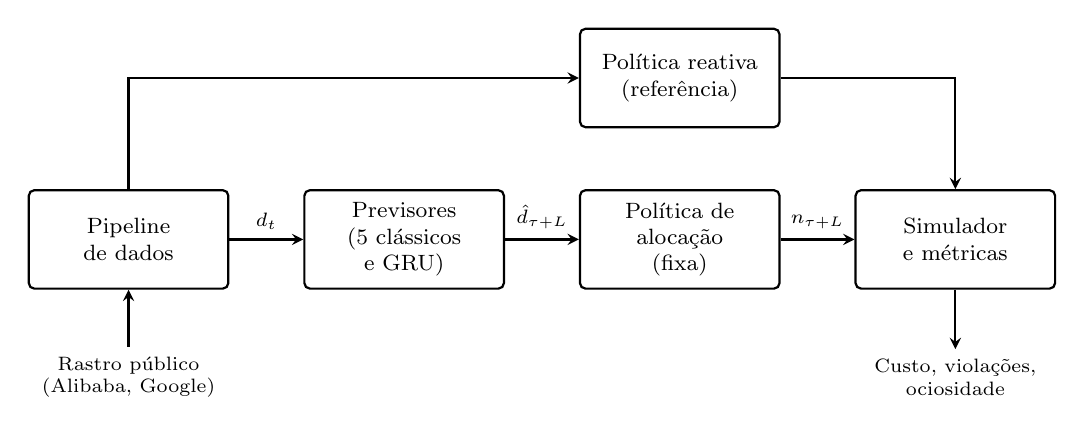
\begin{tikzpicture}[
    >=stealth, thick,
    comp/.style={draw, rounded corners=2pt, align=center, minimum height=1.25cm,
                 text width=2.3cm, font=\footnotesize},
    dado/.style={align=center, font=\scriptsize, text width=2.2cm},
]
\node[comp] (dados) at (0,0)    {Pipeline de dados};
\node[comp] (prev)  at (3.5,0)  {Previsores\\(5 clássicos e GRU)};
\node[comp] (pol)   at (7.0,0)  {Política de alocação\\(fixa)};
\node[comp] (sim)   at (10.5,0) {Simulador e métricas};
\node[dado] (raw)   at (0,-1.75)   {Rastro público\\(Alibaba, Google)};
\node[dado] (res)   at (10.5,-1.75) {Custo, violações,\\ociosidade};
\node[comp] (reat)  at (7.0,2.05) {Política reativa\\(referência)};
\draw[->] (raw)  -- (dados);
\draw[->] (dados) -- node[above, font=\scriptsize] {$d_t$} (prev);
\draw[->] (prev)  -- node[above, font=\scriptsize] {$\hat{d}_{\tau+L}$} (pol);
\draw[->] (pol)   -- node[above, font=\scriptsize] {$n_{\tau+L}$} (sim);
\draw[->] (sim)   -- (res);
\draw[->] (dados.north) |- (reat.west);
\draw[->] (reat.east) -| (sim.north);
\end{tikzpicture}
\caption{Arquitetura da solução proposta. A política de alocação é a mesma para todos os previsores; a política reativa recebe a demanda observada diretamente, sem previsão.}
\label{fig:arquitetura}
\end{figure}

\textbf{Pipeline de dados.} Converte um rastro público de \textit{cluster} em uma série de demanda com intervalos de cinco minutos, expressa em máquinas equivalentes totalmente utilizadas (utilização média de processador das $N$ máquinas, dividida por 100 e multiplicada por $N$).

\textbf{Previsores.} Cinco métodos tradicionais (ingênuo, média móvel, sazonal ingênuo, Holt-Winters e ARIMA; Seção~\ref{subsec:estatisticos}) e uma GRU univariada que, a partir das últimas seis horas, prevê todos os horizontes de uma só vez (estratégia direta; Seção~\ref{subsec:recorrentes}). Todos compartilham uma interface que só dá acesso ao histórico anterior à origem da previsão.

\textbf{Política de alocação.} Aplica uma margem de segurança $m$ sobre a demanda prevista (Equação~\ref{eq:alocacao-margem}). Como referências, há uma política reativa no estilo do \textit{Horizontal Pod Autoscaler} do Kubernetes (Equação~\ref{eq:hpa}) \cite{kubernetes2024hpa}, o dimensionamento fixo pelo pico do treino e um oráculo que conhece a demanda futura.

\textbf{Simulador e métricas.} Reproduz, intervalo a intervalo, um centro de dados com instâncias homogêneas e atraso de provisionamento, contabilizando as métricas da Seção~\ref{subsec:metricas}.

A decisão metodológica central é manter a política de alocação \textbf{fixa} e variar apenas o previsor. Assim, qualquer diferença de custo ou de violações entre duas configurações pode ser atribuída à previsão, e não à regra de decisão.

\section{Objetivos}
\label{sec:objetivos-especificos}

\subsection{Objetivo geral}

Avaliar, em um centro de dados simulado alimentado por rastros públicos de \textit{clusters} reais, a redução de custo operacional obtida pela alocação proativa guiada por uma rede neural recorrente, em comparação com métodos tradicionais de previsão submetidos à mesma política e com uma política reativa, para limites fixos de violação de SLA.

\subsection{Questões de pesquisa}
\label{subsec:questoes}

\begin{description}[leftmargin=1.2cm, style=nextline]
    \item[QP1] Para um mesmo limite de violações $\varepsilon$, a alocação guiada pela rede neural tem custo menor do que a guiada pelos métodos tradicionais? De quanto é a diferença?
    \item[QP2] Um previsor com menor erro (RMSE, MAE) leva necessariamente a uma alocação mais barata no ponto de operação?
    \item[QP3] Qual é o ganho da alocação proativa em relação à reativa, e como ele varia com o atraso de provisionamento $L$?
    \item[QP4] As conclusões obtidas no rastro da Alibaba se mantêm no rastro do Google?
\end{description}

\subsection{Objetivos específicos}

\begin{enumerate}[label=\textbf{OE\arabic*}, leftmargin=1.4cm]
    \item \textbf{Dados:} agregar o Alibaba Cluster Trace de 2018 \cite{alibaba2018trace} em série de 5 minutos, com tratamento de lacunas, divisão cronológica e relatório de qualidade.
    \item \textbf{Previsores:} implementar os seis previsores e avaliá-los por MAE, RMSE, MAPE, viés e taxa de subestimação em cada horizonte.
    \item \textbf{Simulador e políticas:} implementar o simulador e as políticas da Seção~\ref{sec:solucao} (Equação~\ref{eq:politica-preditiva}), validados por testes automatizados.
    \item \textbf{Custo e violações (QP1, QP3):} obter os pontos de operação para $\varepsilon = 1\%$ e $5\%$ (Equação~\ref{eq:calibracao}) e as curvas de custo contra violações.
    \item \textbf{Erro e custo (QP2):} confrontar o erro da previsão de horizonte $h = L$ com o custo no ponto de operação.
    \item \textbf{Sensibilidade (QP3):} medir o efeito do atraso de provisionamento $L$ sobre os pontos de operação.
    \item \textbf{Robustez:} repetir o treinamento da GRU com várias sementes e avaliar em várias janelas de teste, reportando média e dispersão.
    \item \textbf{Replicação (QP4):} aplicar o mesmo protocolo ao Google Cluster Trace de 2019 \cite{wilkes2020google}, alterando apenas a leitura dos dados.
    \item \textbf{Reprodutibilidade:} manter código e configurações em repositório público \cite{rosas2026repo}, regenerando todas as tabelas e figuras com um único comando.
\end{enumerate}

\section{Escopo do sistema}
\label{sec:escopo-sistema}

O sistema é um \textbf{ambiente de simulação e avaliação}, e não um autoescalador para produção. Recebe um rastro de utilização e um arquivo de configuração e produz tabelas e figuras com as métricas de previsão e de alocação; nenhum parâmetro é fixado no código. A Tabela~\ref{tab:parametros} resume os parâmetros do protótipo construído no Projeto Final I, que serão mantidos no Projeto Final II, salvo os ajustes decorrentes de OE6 a OE8.

\begin{table}[htbp]
\centering
\caption{Parâmetros do protocolo experimental adotados no protótipo.}
\label{tab:parametros}
\footnotesize
\begin{tabularx}{\textwidth}{>{\raggedright\arraybackslash}X >{\centering\arraybackslash}p{1.7cm} >{\raggedright\arraybackslash}p{5.6cm}}
\toprule
\textbf{Parâmetro} & \textbf{Símbolo} & \textbf{Valor} \\
\midrule
Intervalo de agregação & $\Delta$ & 5 minutos \\
Divisão cronológica (treino/validação/teste) & -- & 60\% / 20\% / 20\% \\
Horizontes de previsão avaliados & $h$ & 1, 2, 3 e 6 intervalos (5 a 30 min) \\
Janela de entrada da GRU & $w$ & 72 intervalos (6 h) \\
Período sazonal (sazonal ingênuo, Holt-Winters) & -- & 288 intervalos (1 dia) \\
Atraso de provisionamento & $L$ & 1 intervalo; 2 na análise de sensibilidade \\
Instâncias no pico do treino & $n_{\mathrm{pico}}$ & 50 \\
Custo por instância e intervalo & $c$ & 1 \\
Número mínimo de instâncias & $n_{\min}$ & 1 \\
Grade de margens (política preditiva) & $m$ & 0 a 0,60, com passo 0,01 \\
Grade de utilizações-alvo (política reativa) & $u^{*}$ & 0,50 a 0,99, com passo 0,01 \\
Tolerância e estabilização (política reativa) & -- & 10\% e 6 intervalos \\
Limites de violação & $\varepsilon$ & 1\% e 5\% \\
\bottomrule
\end{tabularx}
\end{table}

Valem as simplificações do Capítulo~\ref{cap:situacao-atual}: demanda de processador agregada, capacidade em instâncias homogêneas e violação de SLA sempre que a demanda de um intervalo excede a capacidade. A memória não restringe a alocação, pois sua utilização agregada no rastro da Alibaba varia pouco. Os itens fora do escopo são os da Seção~\ref{sec:escopo}.

\section{Usuários e situações apoiadas}
\label{sec:usuarios}

O ambiente se destina a pesquisadores e a engenheiros responsáveis pelo planejamento de capacidade que precisam decidir se a adoção de um previsor mais complexo se paga em custo de infraestrutura. Ele apoia três situações: comparar previsores sob um mesmo limite de violações antes de levá-los à produção; estimar o custo de operar com um dado nível de serviço e atraso de provisionamento; e estender a avaliação a novos previsores, políticas ou rastros, o que exige apenas implementar a interface comum do componente correspondente.

\section{Avanços em relação às soluções existentes}
\label{sec:avancos}

Os trabalhos de previsão comparam vários modelos, mas apenas por métricas de erro \cite{xu2022esdnn, rossi2023forecasting, agullo2025enhancing}, enquanto os que acoplam previsão e alocação usam um único previsor, comparado com políticas reativas \cite{calheiros2015arima, pan2023magicscaler} (Seção~\ref{sec:comparativo}). Em relação a esse cenário, o trabalho busca:

\begin{itemize}
    \item \textbf{Comparação controlada:} previsores do ingênuo à rede neural sob a mesma política, simulador e dados, combinação ausente na Tabela~\ref{tab:comparativo}.
    \item \textbf{Avaliação pelo custo a um mesmo nível de serviço:} com instâncias discretas e atraso de provisionamento, o que capta a assimetria entre superestimar e subestimar a demanda, diferentemente de \citeonline{rossi2023forecasting}.
    \item \textbf{Ligação explícita entre erro e custo:} a QP2 testa a hipótese, implícita na literatura e posta em dúvida por \citeonline{agullo2025enhancing}, de que menor erro implica melhor alocação.
\end{itemize}

\noindent Todo o experimento usa rastros públicos e código aberto, ao contrário de avaliações com dados privados \cite{pan2023magicscaler}. O trabalho não propõe uma nova arquitetura nem busca superar o estado da arte em erro de previsão: a GRU é deliberadamente simples. A contribuição está em medir o valor operacional da previsão.

\section{Itens a serem implementados e apresentados à banca}
\label{sec:entregaveis}

A Tabela~\ref{tab:entregaveis} relaciona os itens a serem entregues e sua situação ao fim do Projeto Final I. O protótipo já cobre o \textit{pipeline} completo, dos dados brutos às curvas de custo contra violações; o que foi realizado e as dificuldades encontradas são discutidos no Capítulo~\ref{cap:plano-acao}.

\begin{table}[htbp]
\centering
\caption{Itens a serem implementados e situação ao fim do Projeto Final I.}
\label{tab:entregaveis}
\footnotesize
\begin{tabularx}{\textwidth}{>{\raggedright\arraybackslash}X >{\centering\arraybackslash}p{1.6cm} >{\raggedright\arraybackslash}p{5.2cm}}
\toprule
\textbf{Item} & \textbf{Objetivo} & \textbf{Situação no PF~I} \\
\midrule
\textit{Pipeline} de dados & OE1 & Implementado \\
Previsores & OE2 & Implementado \\
Simulador e políticas & OE3 & Implementado \\
Experimentos de custo, violações e erro contra custo & OE4, OE5 & Preliminar (uma semente, uma janela de teste) \\
Análise de sensibilidade & OE6 & Parcial ($L = 1$ e $L = 2$) \\
Avaliação robusta & OE7 & Previsto para o PF II \\
Replicação no Google & OE8 & Previsto para o PF II \\
Repositório reprodutível & OE9 & Implementado; a ser mantido \\
Relatório final e apresentação & -- & Previsto para o PF II \\
\bottomrule
\end{tabularx}
\end{table}

Na defesa, serão apresentados: (i) as curvas de custo contra violações e os pontos de operação de todos os previsores e da política reativa, nos dois rastros; (ii) a comparação entre a ordenação dos previsores por erro e por custo; (iii) a análise de sensibilidade ao atraso de provisionamento; e (iv) a regeneração dos resultados a partir dos dados brutos pelo repositório.

Duas extensões, condicionadas ao cronograma e fora do compromisso de entrega, podem ser avaliadas no mesmo arcabouço: a previsão multivariada com memória como entrada adicional, nos moldes do esDNN \cite{xu2022esdnn}, e a substituição da margem fixa por um quantil previsto pela rede \cite{rossi2023forecasting, pan2023magicscaler}.
  \chapter{Plano de ação}
\label{cap:plano-acao}
  \chapter{Cronogramas}
\label{cap:cronogramas}
  %% ...
  \bibliographystyle{abnt-alf} % \bibliographystyle{abnt-num}
  \bibliography{main}
\end{document}